\section{Theory}\label{sec:theory}
% \paragraph{Anisotropy} of photon distribution would not be present, if there is thermal equilibrium among states. But equilibrium is not achieved in cascaded \gag, since the state of firstly emitted (firstly detected) photon constraints the angular momentum distribution of intermediate state because of angular momentum conservation\cite{descr}.

\paragraph{Angular correlation} of gamma rays of multipole moments $L_{1,2}$ from \gag cascade $I_i \rightarrow I \rightarrow I_f$ is defined as
\begin{equation}
   W(\theta) = 1 + \sum_{k=2, \; \text{even}}^{k_\text{max}} A_{kk} P_k (\cos \theta)
\end{equation}
with $A_{kk}$ (known given the information of nucleus) coefficients, $P_k (\cos \theta)$ the Legendre polynomials, and $k_\text{max} = \text{min}(2I, 2L_1, 2L_2)$\cite{siegbahn}. Alternatively, equivalent definition is sometimes used~\cite{deutsch}
\begin{equation}
   W(\theta) = 1 + \sum_{1}^{l} a_i \cos^{2i} \theta
\end{equation}

\paragraph{Coefficient $A_{kk}$} is determined, generally with mixed multipole components $L'_n$ and $L_n$ ($n=1,2$), by
\begin{align}
   A_{kk} &= A_k(L_1 L_1' I_i I) A_k(L_2 L'_2 I_f I) \\
   A_k(L_n L'_n I_{i,f} I) &= \frac{F_k(L_n L_n I_{i,f} I) + 2 \delta_1(\gamma) F_k (L_n L'_n I_{i,f} I) + \delta_1^2(\gamma) F_{k}(L'_n L'_n I_{i,f} I)}{1 + \delta^2_1 (\gamma)} \\
   F_k(L L' I' I) &= (-1)^{I'+I-1} \left[ (2L + 1) (2L' + 1)(2I+1) (2k+1) \right]^{1/2} \notag \\
     & \quad \times \begin{pmatrix} L & L' & k \\ 1 & -1 & 0 \end{pmatrix} \begin{Bmatrix} L & L' & k \\ I & I & I'\end{Bmatrix} \\
   \delta_1 (\gamma) &= \frac{\braket{I | L'_1 \pi'_1 | I_{i,f}}}{ \braket{I | L_1 \pi_1 | I_{i,f}}}
\end{align}
with round brackets being $3j$-symbols and curly brackets $6j$-symbols\cite{siegbahn}. Their value can be easily found tabulated, e.g. in \cite{STEVENSON2002853} and \cite{369j}. $\delta_{n}(\gamma)$ quantifies the mixing of two multipole moments and should be determined by some other methods. If we assume $L'_n = L_n + 1$ (this is reasonable because of selection rules), then there are $7$ quantum numbers to nail down the coefficients: $I_i, I, I_f, \delta_{1,2}, L_{1,2}$\cite{siegbahn}.

\paragraph{Example} with $0 \rightarrow 1 \rightarrow 0$ \gag cascade. Since the first and last states are of spin $0$, the multipolarities of emitted photon must be $1$, thus dipole-dipole radiation. According to~\cite{deutsch}
\begin{equation}
   W(\theta) = 1 + \cos^{2}(\theta)
   \label{math:W010}
\end{equation}

Plot of this angular correlation can be found in figure \ref{W010}.
\begin{figure}[ht]
   \centering
   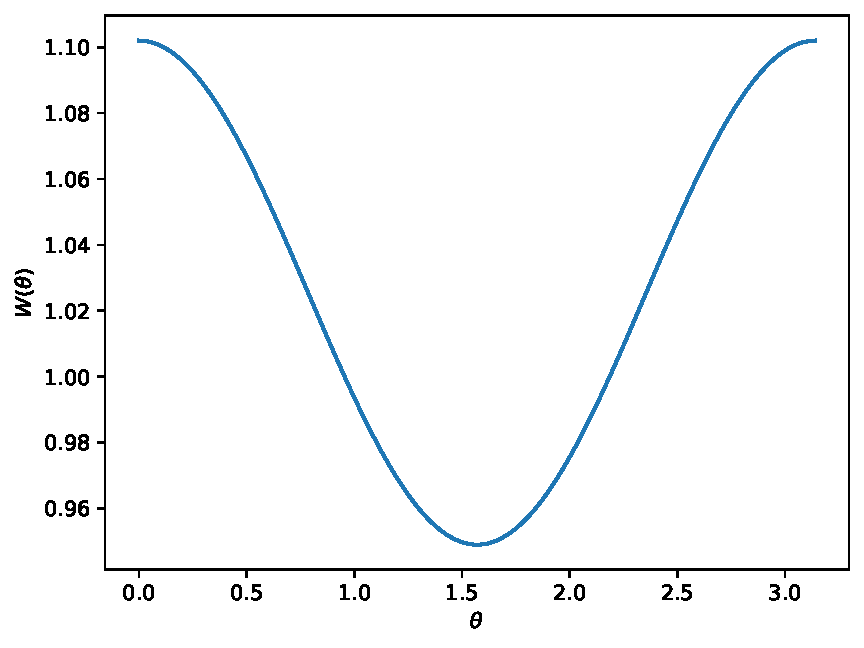
\includegraphics[width=0.5\linewidth]{010.pdf}
   \caption{Angular correlation of hypothetical 010 cascade}%
   \label{W010}
\end{figure}

\paragraph{Hyperfine structure} can have influence on the angular correlation, since with quantization axis along the direction of first photon the first photon will cause transitions among the $m$-states. Thus in the end, the direction of second photon is altered. The perturbed angular correlation is given as
\begin{equation}
   W(k_1, k_2, t) = \sum_{m_i, m_f, m_a, m'_a} \braket{m_f | H_2 \Lambda(t) | m_a} \braket{m_a | H_1 | m_i} \braket{m_f | H_2 \Lambda(t) | m'_a}^* \braket{m'_a | H_1 | m_i}^*
\end{equation}
where $H_{1,2}$ represents the interaction between nucleus and radiation field and $\Lambda(t)$ is an unitary operator describing influence of extranuclear perturbation. $k_1$ and $k_2$ are wave vector of photons.
~\cite{siegbahn}.


\paragraph{Information} can be obtained from measurement of \gag angular correlations (without extranuclear perturbation): spin angular momenta of excited states, the multipole orders, and the relative multipole composition of radiative transitions\cite{RAWilson}. With extranuclear perturbation, we can in addition extract $g$-factor and quadrupole momentum of intermediate state. Internal fields of solids, liquids, and metal crystals can be investigated. And some changes in atomic shell is possible to study~\cite{siegbahn}.
